\section{Spin-Statistics Theorem, Quantizing the Dirac Lagrangian}
\subsection{Exchange statistics}
We have seen that a general representation of the Lorentz group on a field takes the form:
\begin{equation}
    \psi(x) \to \psi'(x) = U(\Lambda)^{-1}\psi(x)U(\Lambda) = D(\Lambda)\psi(\Lambda^{-1}x)
\end{equation}
where $D(\Lambda)$ is the finite-dimensional representation of the Lorentz group acting on the indices $\psi_a$. In other words, it acts on the coordinate and then also acts on the fields themselves via a matrix.

We have also seen that for half-integer spin representations, $D(2\pi) = -1$ (i.e. the matrix that realizes a $2\pi$ rotation of spinors gives negative of the identity). We saw this in the case of Weyl and Dirac spinors/fermions, but this is much more general; any half-integer representation (any where $\v{J} = \v{J}_+ + \v{J}_-$ sums to a half-integer) of $SU(2)$ has this property. This is a hint towards the spin-statistics theorem and will be an ingredient in its proof. We will show that this requires that the corresponding field has fermionic statistics, i.e. obey the anticommutation relations:
\begin{equation}
    \set{\hat{\psi}(\v{x}), \hat{\psi}(\v{y})} = 0 \quad (\v{x} \neq \v{y})
\end{equation}
These operators create states/wavefunctions that are antisymmetric under exchange of identical particles, i.e.:
\begin{equation}
    \ket{\ldots, \v{x}, \v{y}, \ldots} = -\ket{\ldots, \v{y}, \v{x}, \ldots}.
\end{equation}
Note that $\pm$ are the only options (at least, in 3+1d). Because the particles are indistinguishable, the states have to be equivalent; they can at most differ by a phase:
\begin{equation}
    \ket{\ldots, \v{x},\v{y}, \ldots} = e^{i\phi}\ket{\ldots, \v{y}, \v{x}, \ldots}
\end{equation}
But exchanging twice is continuously deformable to doing nothing (we can use the ``third dimension'' to continuously deform this double exchange to the identity identity), so $e^{2i\phi} = 1$ which implies $e^{i\phi} = \pm 1$. But note that being in 3-d is crucial; in 2D we are confined to the plane, so if we try to take our particles and deform the double exchange to the identity, we can only accomplish this by making the particles hit each other. 

So in summary, in 3+1d we can only have bosonic ($+1$) or fermionic ($-1$) statistics. But in 2+d1 we can in general have $e^{2i\phi} \neq 1$, and have ``any'' statistics $e^{i\phi}$, i.e. we have ``anyons''. These are not fundamental particles (because we don't live in 2d) but emerge in condensed matter systems such as in the fractional quantum Hall effect and toric code.

\subsection{Proof of spin-statistics in 3+1d (almost)}

\begin{center}
    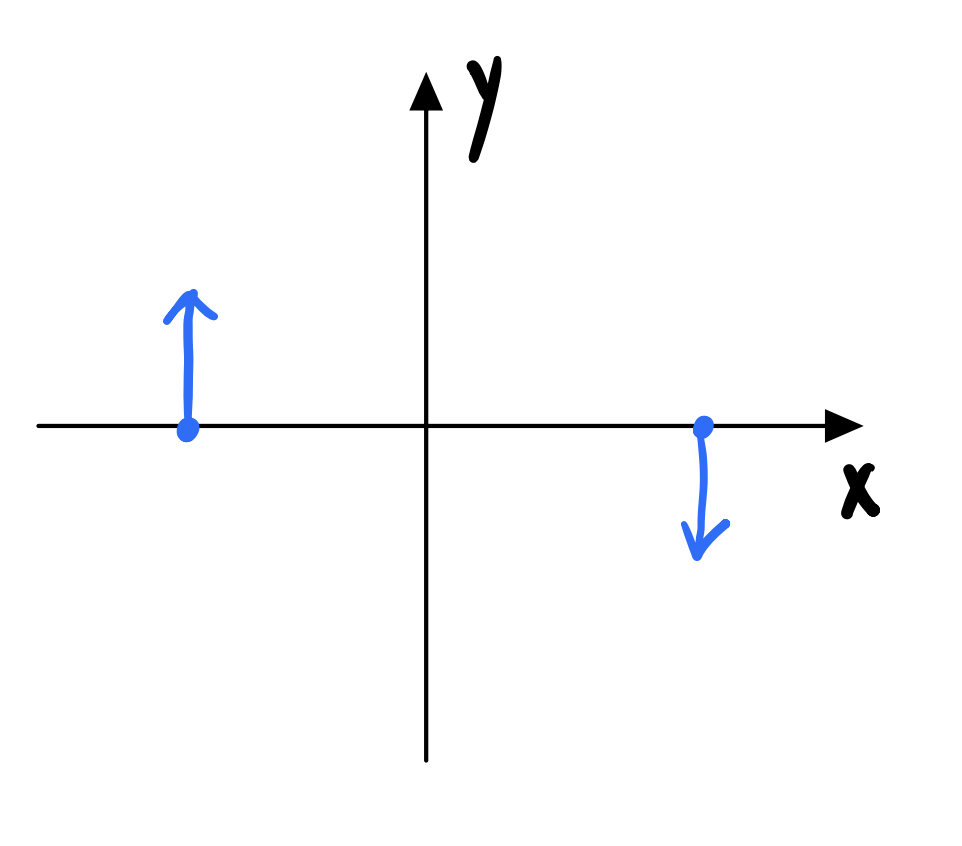
\includegraphics[scale=0.4]{Lectures/Images/lec3-twospinors.png}
\end{center}

We consider a two-point function involving two fermionic fields in the vacuum:
\begin{equation}
    G(x) = \bra{0}D(\pi)\hat{\psi}(\v{x})\hat{\psi}(-\v{x})\ket{0}
\end{equation}
Let us introduce $\hat{U}(\Lambda)\hat{U}(\Lambda)^{-1}$ for $\hat{U}(\Lambda) = \hat{R}$ a rotation by $\pi$. We use the Lorentz invariance of the vaccum, i.e. $\hat{U}(\Lambda)\ket{0} = \ket{0}$.
\begin{equation}
    \begin{split}
        G(x) &= \bra{0}\hat{U}(\Lambda)\hat{U}(\Lambda)^{-1}D(\pi)\hat{\psi}(\v{x})\hat{U}(\Lambda)\hat{U}(\Lambda)^{-1}\hat{\psi}(-\v{x})\hat{U}(\Lambda)\hat{U}(\Lambda)^{-1}\ket{0} 
        \\ &= \bra{0}\hat{U}(\Lambda)^{-1}D(\pi)\hat{\psi}(\v{x})\hat{U}(\Lambda)\hat{U}(\Lambda)^{-1}\hat{\psi}(-\v{x})\hat{U}(\Lambda)\ket{0}
        \\ &= \bra{0}D(\pi)D(\pi)\hat{\psi}(-\v{x})D(\pi)\hat{\psi}(\v{x})\ket{0}
        \\ &= \bra{0}D(2\pi)\hat{\psi}(-\v{x})D(\pi)\hat{\psi}(\v{x})\ket{0}
        \\ &= -\bra{0}\hat{\psi}(-\v{x})D(\pi)\hat{\psi}(\v{x})\ket{0}
    \end{split}
\end{equation}
where in the third equality we note that $\hat{U}(\Lambda)^{-1}\hat{\psi}(\v{x})\hat{U}(\Lambda) = D(\pi)\hat{\psi}(-\v{x})$ and in the final equality we use that $D(2\pi) = -1$ for fermions (note that $D(\pi)$ is just a matrix acting on the indices of $\hat{\psi}$ and so we can move it around freely in the expression). This establishes that the $\psi$ operators have fermionic statistics.

One thing we swept under the rug is the possibility that $G(x) = 0$. This comes from the CPT theorem; invariance under charge/parity/time-reversal symmetry follows that $G(x) > 0$. \qed

Rio note: Asked whether it matters that we only showed it for $\pm \v{x}$ - answer was that it suffices to show it for one correlator. I think maybe you could argue this (from spatial translation/rotation invariance) that all possible coordinate pairs would reduce to the $\pm \v{x}$ case?

Also, note that there are different available proofs of spin-statistics, and each offer a different perspective; see Schwartz for more details and insight.

\subsection{Review of quantizing the free scalar}
We follow Srednicki 37-39 for this discussion.

We recall the Dirac Lagrangian we had constructed:
\begin{equation}
    \mathcal{L} = i\bar{\Psi}\slashed{\p}\Psi - m \bar{\Psi}\Psi
\end{equation}
where $\Psi = \m{\psi_L \\ \psi_R}$ and $\slashed{\p} = \p_\mu \gamma^\mu$ with $\gamma$ matrices:
\begin{equation}
    \gamma^\mu = \m{0 & \sigma^\mu \\ \bar{\sigma}^\mu & 0}
\end{equation}
so:
\begin{equation}
    \slashed{\p} = \m{0 & 0 & \p_0 + \p_3 & \p_1 - i\p_2 \\ 0 & 0 & \p_1 + i\p_2 & \p_0 - \p_3 \\ \ldots & \ldots & 0 & 0 \\ \ldots & \ldots & 0 & 0}.
\end{equation}
We want to quantize this Lagrangian, but let us first review how we quantized the free scalar. For the free scalar that we had the action:
\begin{equation}
    S = -\frac{1}{2}\int (\p\phi)^2 + m^2\phi^2
\end{equation}
the conjugate momenta:
\begin{equation}
    \pi(x) = \frac{\delta S}{\delta \dot{\phi}} = \dot{\phi}
\end{equation}
which obeyed the canonical Poisson bracket relation:
\begin{equation}
    \set{\phi(\v{x}), \pi(\v{y})}_{\text{PB}} = \delta^3(\v{x} - \v{y})
\end{equation}
which we promoted to a commutator relation of operators via canonical quantization:
\begin{equation}
    [\hat{\phi}(\v{x}), \hat{\Pi}(\v{y})] = i\delta^3(\v{x} - \v{y}).
\end{equation}
We had the Hamiltonian, which we quantized and diagonalized:
\begin{equation}
    \begin{split}
        H &= \int \Pi \dot{\phi} - \mathcal{L} 
        \\ &= \int d^3x \frac{1}{2}\Pi^2 + \frac{1}{2}(\nabla \phi)^2 + \frac{1}{2}m^2\phi^2 = \int \frac{d^3k}{(2\pi)^3}\frac{1}{2}\abs{\Pi_\v{k}}^2 + \frac{1}{2}(\v{k}^2 + m^2)\abs{\phi_\v{k}}^2 
        \\ &= \int \frac{d^3k}{(2\pi)^32\e_\v{k}}\e_{\v{k}}a^\dag_{\v{k}}a_{\v{k}}
    \end{split}
\end{equation}
with:
\begin{equation}
    \begin{split}
        a_\v{k} = \e_{\v{k}}\phi_{\v{k}} + i\Pi_{\v{k}}
        \\ a_\v{k}^\dag = \e_{\v{k}}\phi_{-\v{k}} - i\Pi_{-\v{k}}
    \end{split}
\end{equation}
and so:
\begin{equation}
    \phi_{\v{k}} = \frac{1}{2\e_{\v{k}}}(a_{\v{k}} + a_{\v{k}}^\dag)
\end{equation}
so we found the full time evolution of the fields:
\begin{equation}
    \phi(t, \v{x}) = \int \frac{d^3k}{(2\pi)^32\e_{\v{k}}}(a_\v{k}e^{i\v{k} \cdot \v{x}} + a^\dag_{\v{k}}e^{-i\v{k} \cdot \v{x}})
\end{equation}
with $k^0 = \e_{\v{k}} = \sqrt{\v{k}^2 + m^2}$. The Hilbert space of our scalar QFT was Fock space, with:
\begin{equation}
    a_\v{k}\ket{0} = 0 \quad \forall \v{k}
\end{equation}
\begin{equation}
    a^\dag_{\v{k}}\ket{0} = \ket{\v{k}}, a^\dag_{\v{k}_1}a^\dag_{\v{k}_2} = \ket{\v{k}_1, \v{k}_2}, \ldots
\end{equation}

\subsection{Quantizing the Dirac Lagrangian}
With that review under our belt, we want to quantize:
\begin{equation}
    \mathcal{L} = i\bar{\Psi}\gamma^\mu p_\mu \Psi - m\bar{\Psi}\Psi
\end{equation}
so we have the canonical momenta:
\begin{equation}
    \Pi = \frac{\delta S}{\delta \dot{\Psi}} = i\bar{\Psi}\gamma^0 = i\Psi^\dag \gamma^0 \gamma^0 = i\Psi^\dag \implies \Pi_a = i\Psi_a^*
\end{equation}
Thus canonical quantization promotes:
\begin{equation}
    \set{\Psi_a(\v{x}), \Pi_b(\v{y})}_{\text{PB}} = \delta^3(\v{x} - \v{y})\delta_{ab}
\end{equation}
to the commutator:
\begin{equation}
    [\hat{\Psi}_a(\v{x}), \hat{\Pi}_b(\v{y})] = i\delta^3(\v{x} - \v{y})\delta_{ab}.
\end{equation}
The Hamiltonian reads:
\begin{equation}
    H = \Pi\dot{\Psi} - \mathcal{L} = -i\bar{\Psi}\gamma^i\p_i \Psi + m\bar{\Psi}\Psi
\end{equation}

\subsection{General Solution for Dirac Equation}
Let's try to find the most general solution $\Psi(t, \v{x})$ of the Dirac equation:
\begin{equation}
    (i\slashed{\p} - m)\Psi = 0.
\end{equation}
Because $\Psi(x)$ satisfies the Klein-Gordon equation (which follows from the Dirac equation):
\begin{equation}
    (\square + m^2)\Psi = 0
\end{equation}
a general solution will take the form:
\begin{equation}
    \Psi(t, \v{x}) = u(\v{p})e^{ipx} + v(\v{p})e^{-ipx}
\end{equation}
where $u, v$ are 4-component spinors:
\begin{equation}
    u(\v{p}) = \m{u_1(\v{p}) \\ u_2(\v{p}) \\ u_3(\v{p}) \\ u_4(\v{p})}
\end{equation}
and we have the on-shell condition for $p = (p^0, \v{p})$:
\begin{equation}
    p^0 = \e_\v{p} = \sqrt{\v{p}^2 + m^2}.
\end{equation}
But, the solution also has to solve the Dirac equation, which gives us the further condition on the spinors:
\begin{equation}
    0 = (i\slashed{\p} - m)\Psi = (-\slashed{p} - m)u(\v{p})e^{ipx} + (\slashed{p} - m)v(\v{p})e^{-ipx} \implies \begin{cases}
        (\slashed{p} + m)u(\v{p}) = 0
        \\ (\slashed{p} - m)v(\v{p}) = 0
    \end{cases}
\end{equation}
The trick will be to solve these equations in a preferred frame - namely the rest frame, where $ p^\mu_{\text{rest}} = (m, \v{0})$ -  and then boost back to an arbitrary frame $p^\mu = \Lambda^{\mu}_{\sp\nu}p^\nu_{\text{rest}}$:
\begin{equation}
    u(\v{p}) = D(\Lambda)u(\v{0})
\end{equation}
This works because the Dirac equation is Lorentz invariant, but let's check:
\begin{equation}
    \begin{split}
        0 \stackrel{?}{=} (\slashed{p} + m)D(\Lambda)u(\v{0}) &= D(\Lambda)D(\Lambda)^{-1}(\slashed{p} + m)D(\Lambda)u(\v{0}) 
        \\ &= D(\Lambda)(p_\mu D(\Lambda)^{-1}\Gamma^\mu D(\Lambda) - m)u(\v{0})
        \\ &= D(\Lambda)(p_\mu \Lambda^{\mu}_{\sp\nu}\gamma^\nu - m)u(\v{0})
        \\ &= D(\Lambda)(\slashed{p}_{\text{rest}} - m)u(\v{0})
        \\ &= 0.
    \end{split}
\end{equation}
So indeed this strategy works!

In the rest frame we have $p^0_{\text{rest}} = m$ and $p_{0, \text{rest}} = -m$ and so:
\begin{equation}
    \slashed{p}_{\text{rest}} = p_0\gamma^0 = -m\m{0 & \II \\ \II & 0}
\end{equation}
Thus our equation for $u$ is:
\begin{equation}
    m\m{\II & -\II \\ -\II & \II}\m{u_1 \\ u_2 \\ u_3 \\ u_4} = 0
\end{equation}
This implies that $u_1 -u_3 = 0$ and $u_2 -u_4 = 0$. One possible basis for the rest frame solution is therefore:
\begin{equation}
    u_+(\v{0}) = \m{1 \\ 0 \\ 1 \\ 0}, \quad u_-(\v{0}) = \m{0 \\ 1 \\ 0 \\ 1}.
\end{equation}
This basis is convenient because these solutions have a well-defined spin in the $\zhat$-direction (namely $\pm \frac{1}{2}$). Let us do the same for $v$:
\begin{equation}
    m\m{\II & \II \\ \II & \II}\m{v_1 \\ v_2 \\ v_3 \\ v_4} = 0
\end{equation}
This implies that $v_1 + v_3 = 0$ and $v_2 + v_4 = 0$. We then have a basis of solutions:
\begin{equation}
    v_+(\v{0}) = \m{0 \\ 1 \\ 0 \\ -1}, \quad v_-(\v{0}) = \m{-1 \\ 0 \\ 1 \\ 0}
\end{equation}
Now, we boost to get the general solution. What is the Lorentz transformation that takes $p^\mu_{\text{rest}} = (m, \v{0})$ into $p^\mu = (\sqrt{m^2 + \v{p}^2}, \v{p})$? It is clear that we must boost in the $\hat{\v{p}} = \frac{\v{p}}{\abs{\v{p}}}$ direction, so we want the boost $e^{i\eta \hat{\v{p}} \cdot \v{k}}$ by an amount (rapidity) $\eta = \sinh(\frac{\abs{\v{p}}}{m})$. What is then $D(\v{k})$ (representation of boosts on spinors)? This we can construct by recalling that $\v{k} = \frac{\v{J}_+ - \v{J}_-}{i}$ so then:
\begin{equation}
    K_i = \m{\frac{i}{2}\sigma_i & 0 \\ 0 & -\frac{i}{2}\sigma_i}.
\end{equation}
So, in summary:
\begin{equation}
    u(\v{p}) = D(\Lambda)u(\v{0}) = e^{i\eta \hat{p}^iK_i}
\end{equation}
with the $\eta, K_i$ as described the above. There are solutions for $u_\pm, v_\pm$. At the end of the day, a general solution to the Dirac equation takes the form of a most general linear combination of these solutions:
\begin{equation}
    \Psi(t, \v{x}) = \sum_{s = \pm} \int \frac{d^3p}{(2\pi)^32\e_{\v{p}}}[b_s(\v{p})u_s(\v{p})e^{ipx} + d_s^\dag(\v{p})v_s(\v{p})e^{-ipx}]
\end{equation}
Classically, $b, d^\dag$ are coefficients, but after we finish quantizing the theory on Thursday we will see that they play similar roles to the creation/annihilation operators as in the scalar case, and they will create/annihilate spin-1/2 particles. Moreover, we will see that they have to come with a particle-pair; the Dirac equation solutions predict the existence of antiparticles! Historically, this was how the positron (the antiparticle of the electron) was predicted.